%%%%%%%%%%%%%%%%%%%%%%%%%%%%%%%%%%%%%%%%%%%%%%%%%%%%%%%%%%%%%%%%%%%%%%%%%%%%%%%%%%
\begin{frame}[fragile]\frametitle{}
\begin{center}
{\Large Concepts}
\end{center}
\end{frame}


%%%%%%%%%%%%%%%%%%%%%%%%%%%%%%%%%%%%%%%%%%%%%%%%%%%%%%%%%%%
\begin{frame}[fragile]\frametitle{Overview}

Overview of traditional RAG and two typical GraphRAG workflows.

    \begin{itemize}
        \item Non-graph RAG organizes the corpus into chunks, ranks them by similarity, and retrieves the most relevant text for generating responses.
        \item Knowledge-based GraphRAG extracts detailed knowledge graphs from the corpus using entity recognition and relation extraction, offering fine-grained, domain-specific information.
        \item Index-based GraphRAG summarizes the corpus into high-level topic nodes, which are linked to form an index graph, while the fact linking maps topics to text.
    \end{itemize}
	
	{\tiny (Ref: Awesome-GraphRAG (GraphRAG Survey))}
	
\end{frame}

% %%%%%%%%%%%%%%%%%%%%%%%%%%%%%%%%%%%%%%%%%%%%%%%%%%%%%%%%%%%%%%%%%%%%%%%%%%%%%%%%%%
% \begin{frame}[fragile]\frametitle{}
% \begin{center}
% {\Large Knowledge Graphs}
% \end{center}
% \end{frame}

%%%%%%%%%%%%%%%%%%%%%%%%%%%%%%%%%%%%%%%%%%%%%%%%%%%%%%%%%%%
\begin{frame}[fragile]\frametitle{Btw, What is Knowledge Graph?}
    \begin{block}{Definition}
A Knowledge Graph is a structured way of representing 
information, typically using nodes and edges to depict 
relationships between entities (e.g., people, places, 
things, concepts). 
These entities and their interconnections form a 
graph-like structure, which can be used to model 
complex sets of data and the relationships within that 
data.
    \end{block}
	
	{\tiny (Ref: The GenAI Stack - Andreas Kollegger - Neo4j)}
	
\end{frame}


%%%%%%%%%%%%%%%%%%%%%%%%%%%%%%%%%%%%%%%%%%%%%%%%%%%%%%%%%%%
\begin{frame}[fragile]\frametitle{}

	\begin{center}
	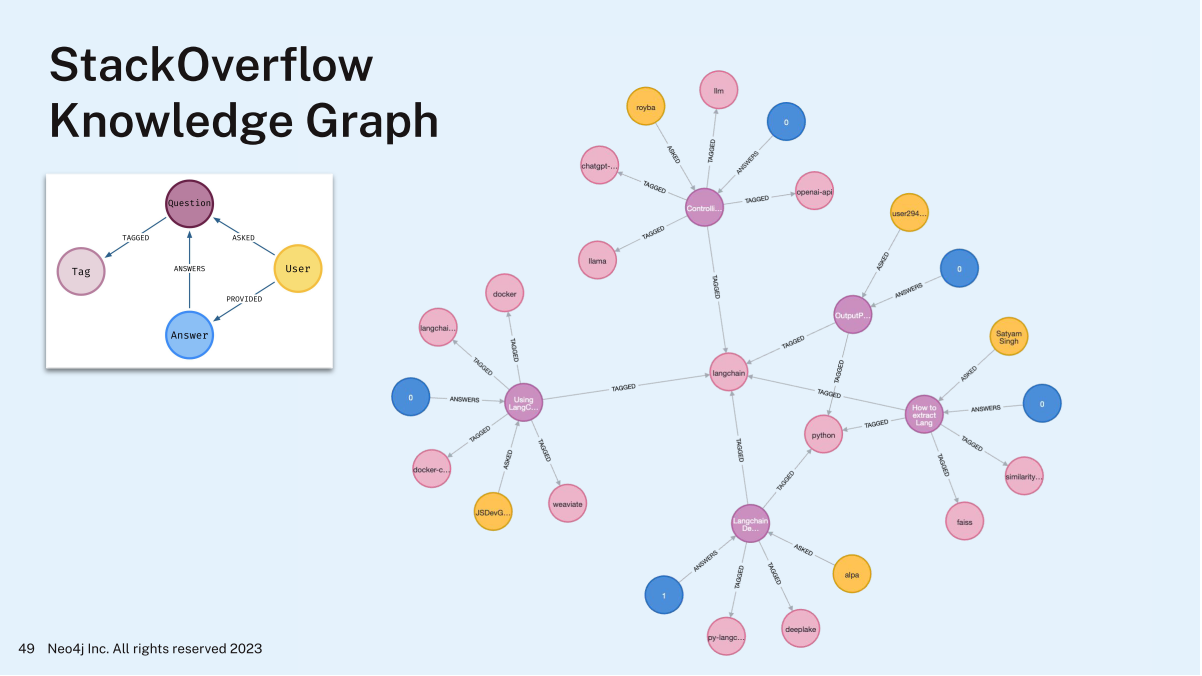
\includegraphics[width=\linewidth,keepaspectratio]{graphrag7}
	\end{center}
	
\end{frame}

% %%%%%%%%%%%%%%%%%%%%%%%%%%%%%%%%%%%%%%%%%%%%%%%%%%%%%%%%%%%
% \begin{frame}[fragile]\frametitle{}

	% \begin{center}
	% 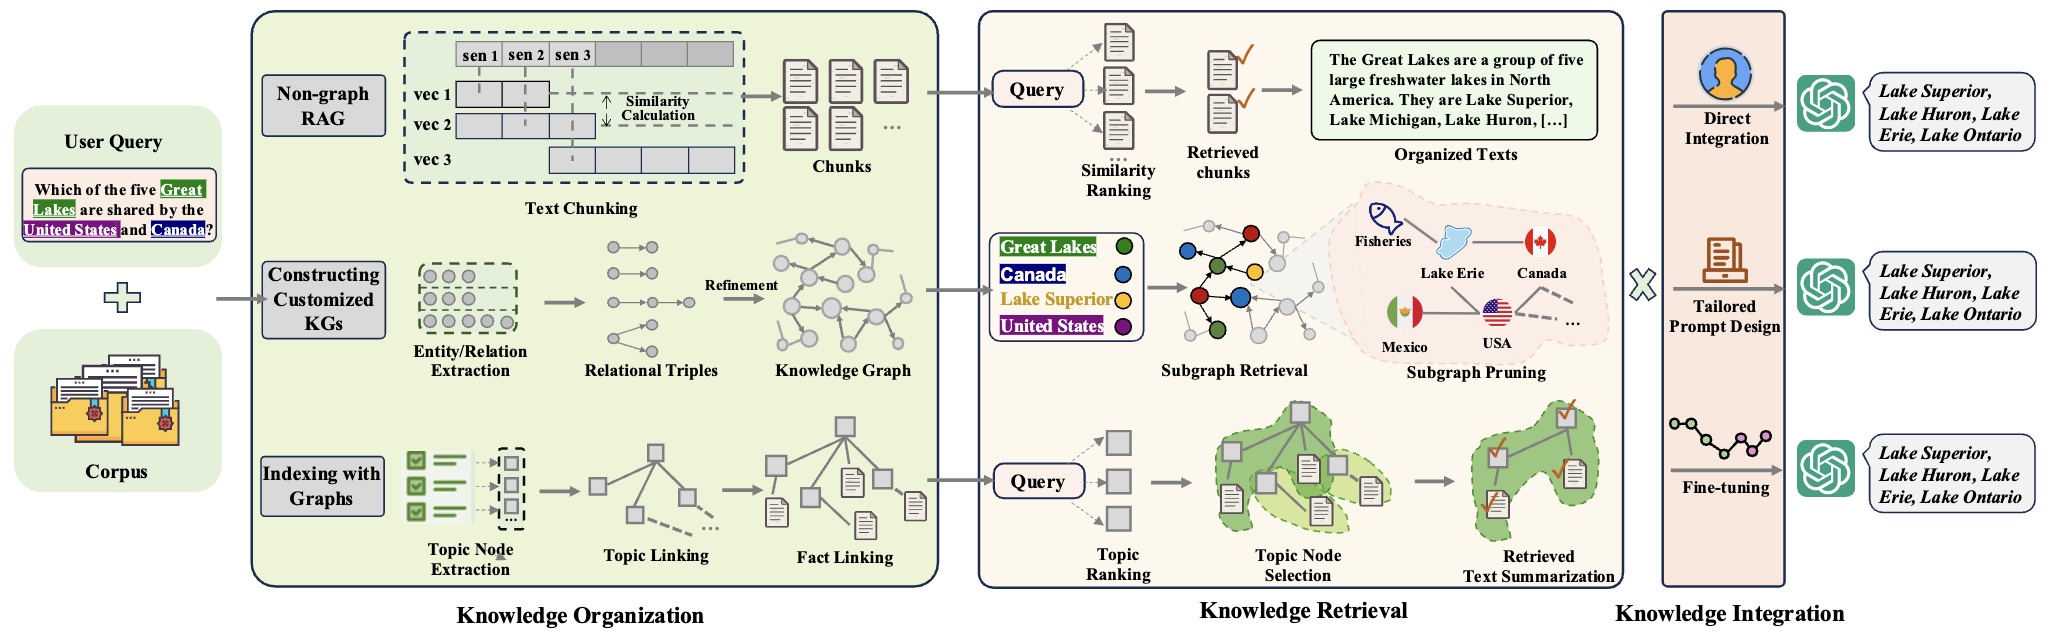
\includegraphics[width=\linewidth,keepaspectratio]{graphrag11}
	% \end{center}
	
% \end{frame}

%%%%%%%%%%%%%%%%%%%%%%%%%%%%%%%%%%%%%%%%%%%%%%%%%%%%%%%%%%%
\begin{frame}[fragile]\frametitle{Graph Construction Economy Principle}
    \begin{itemize}
        \item Complex graphs require significant computational resources.
        \item Trade-off: Performance gains must justify resource investment.
        \item Aim: Maximize performance-to-resource ratio.
    \end{itemize}
\end{frame}


%%%%%%%%%%%%%%%%%%%%%%%%%%%%%%%%%%%%%%%%%%%%%%%%%%%%%%%%%%%%%%%%%%%%%%%%%%%%%%%%%%
\begin{frame}[fragile]\frametitle{}
\begin{center}
{\Large Approaches}
\end{center}
\end{frame}

%%%%%%%%%%%%%%%%%%%%%%%%%%%%%%%%%%%%%%%%%%%%%%%%%%%%%%%%%%%
\begin{frame}[fragile]\frametitle{Cost-Efficient GraphRAG Approach}
    \begin{itemize}
        \item Leverages graphs for RAG without high costs.
        \item Minimizes reliance on LLMs or uses smaller on-premise models.
        \item Structured as a layered graph:
        \begin{itemize}
            \item Ontology Layer – Defines domain structure (fixed or nearly fixed).
            \item Document Layer – Contains chunked documents, similar to a vector DB.
            \item Entity Layer (Optional) – Extracted entities enhance search.
        \end{itemize}
    \end{itemize}
\end{frame}

%%%%%%%%%%%%%%%%%%%%%%%%%%%%%%%%%%%%%%%%%%%%%%%%%%%%%%%%%%%
\begin{frame}[fragile]\frametitle{Challenges in Ontology-Based Graphs}
    \begin{itemize}
        \item Not all datasets belong to a well-defined domain.
        \item Subject Matter Experts (SMEs) may not be available.
        \item Eliminating fixed ontology layer could improve flexibility.
    \end{itemize}
\end{frame}

%%%%%%%%%%%%%%%%%%%%%%%%%%%%%%%%%%%%%%%%%%%%%%%%%%%%%%%%%%%
\begin{frame}[fragile]\frametitle{NLP-Powered Graph Approach}
    \begin{itemize}
        \item Drops the ontology layer for cost-efficiency.
        \item Graph consists of:
        \begin{itemize}
            \item Document Layer – Contains document chunks.
            \item Tokens Layer – Extracted tokens improve search.
        \end{itemize}
        \item NLP reduces dependency on LLMs.
    \end{itemize}
\end{frame}

%%%%%%%%%%%%%%%%%%%%%%%%%%%%%%%%%%%%%%%%%%%%%%%%%%%%%%%%%%%
\begin{frame}[fragile]\frametitle{Data Preprocessing Pipeline}
    \begin{itemize}
        \item Chunking – Splitting documents into segments.
        \item Embedding – Using Hugging Face model for embeddings.
        \item Graph Construction – Built using NetworkX or Neo4j.
        \item Token Extraction – Generates token, bigram, and trigram nodes.
    \end{itemize}
\end{frame}

%%%%%%%%%%%%%%%%%%%%%%%%%%%%%%%%%%%%%%%%%%%%%%%%%%%%%%%%%%%
\begin{frame}[fragile]\frametitle{Indexing and Interconnectivity}
    \begin{itemize}
        \item Tokens are shared across documents, interlinking content.
        \item Need to connect entities using context, logic, and semantics.
        \item Avoid reliance on massive models due to cost constraints.
    \end{itemize}
\end{frame}

%%%%%%%%%%%%%%%%%%%%%%%%%%%%%%%%%%%%%%%%%%%%%%%%%%%%%%%%%%%
\begin{frame}[fragile]\frametitle{Triple Extraction for Graph Optimization}
    \begin{itemize}
        \item Triple extraction improves retrieval efficiency.
        \item Uses a smaller transformer model fine-tuned for this task.
        \item Triplets mapped to token nodes enhance query performance.
        \item Queries traverse graph using triplet relationships.
    \end{itemize}
\end{frame}

%%%%%%%%%%%%%%%%%%%%%%%%%%%%%%%%%%%%%%%%%%%%%%%%%%%%%%%%%%%
\begin{frame}[fragile]\frametitle{Optimizing Graph-Based Retrieval}
    \begin{itemize}
        \item Combines standard RAG with triplet-enhanced retrieval.
        \item Retrieves relevant text chunks and connected triplets.
        \item Improves search relevance and reduces retrieval complexity.
    \end{itemize}
\end{frame}




%%%%%%%%%%%%%%%%%%%%%%%%%%%%%%%%%%%%%%%%%%%%%%%%%%%%%%%%%%%
\begin{frame}[fragile]\frametitle{}

	\begin{center}
	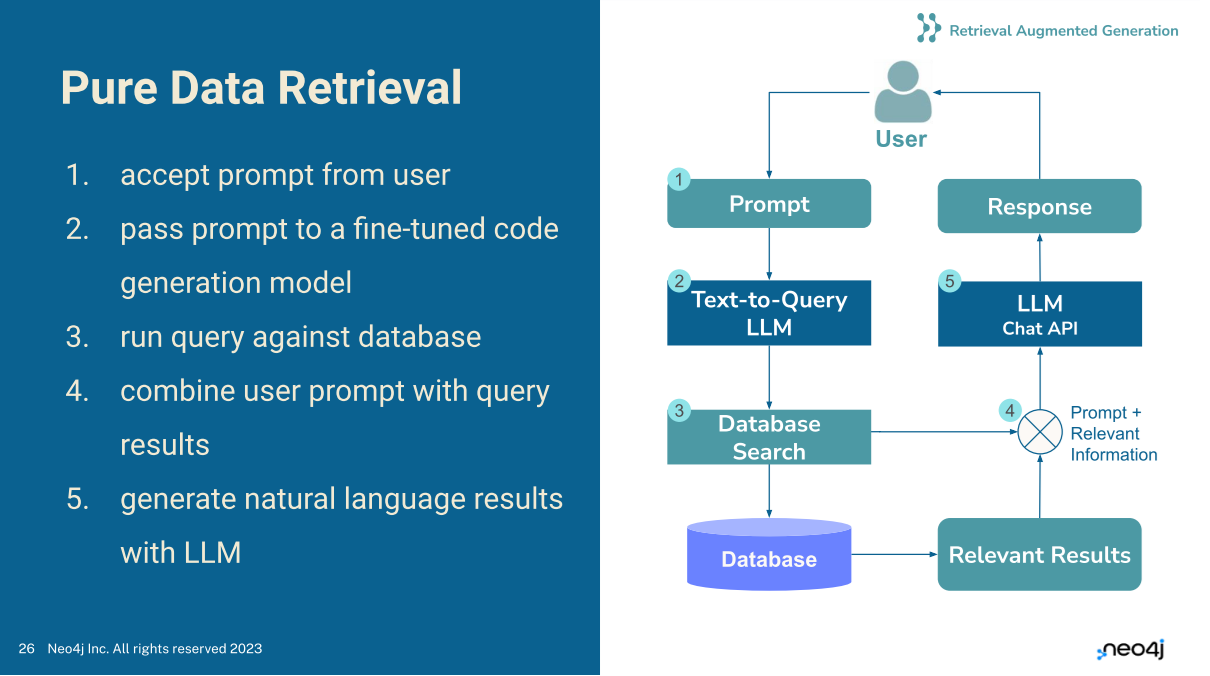
\includegraphics[width=\linewidth,keepaspectratio]{graphrag3}
	\end{center}
	
	
\end{frame}

%%%%%%%%%%%%%%%%%%%%%%%%%%%%%%%%%%%%%%%%%%%%%%%%%%%%%%%%%%%
\begin{frame}[fragile]\frametitle{Challenges}
    \begin{itemize}
        \item Getting it to work at all – generating syntactically correct queries
        \item Getting it to do the right thing – producing meaningful results
        \item Avoiding accidents – mistaken deletion
        \item Preventing malicious intent – SQL injection gone wild
    \end{itemize}
	
	{\tiny (Ref: The GenAI Stack - Andreas Kollegger - Neo4j)}
	
\end{frame}


%%%%%%%%%%%%%%%%%%%%%%%%%%%%%%%%%%%%%%%%%%%%%%%%%%%%%%%%%%%
\begin{frame}[fragile]\frametitle{}

	\begin{center}
	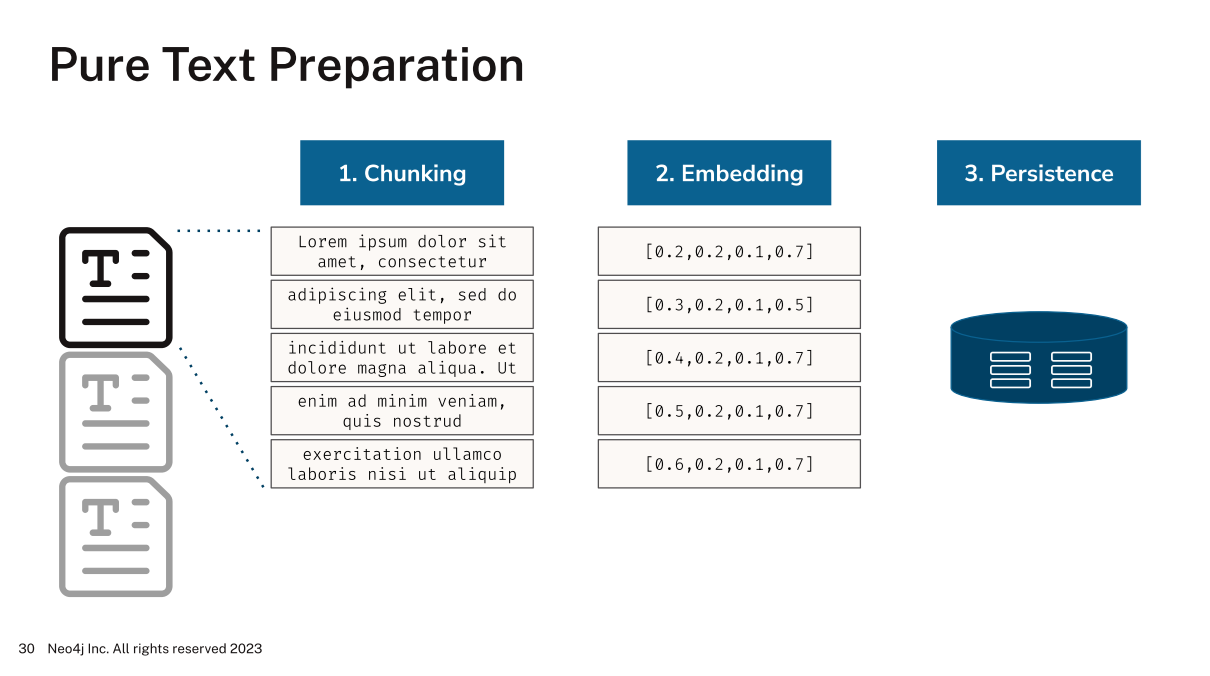
\includegraphics[width=\linewidth,keepaspectratio]{graphrag4}
	\end{center}
	
\end{frame}

%%%%%%%%%%%%%%%%%%%%%%%%%%%%%%%%%%%%%%%%%%%%%%%%%%%%%%%%%%%
\begin{frame}[fragile]\frametitle{Challenges}
    \begin{itemize}
        \item How?
		    \begin{itemize}
				\item pick a chunk method \& size
				\item each chunk is a record
				\item store chunk with metadata
				\item connect each chunk to original document
				\item connect previous/next chunk
		    \end{itemize}
        \item Challenges:
		    \begin{itemize}
				\item what makes a good chunk?
				\item potential chunk duplication
				\item how to re-assemble chunk context?
				\item  what about cross-document chunks?
				\item explaining the relevance
		    \end{itemize}
    \end{itemize}
	
	{\tiny (Ref: The GenAI Stack - Andreas Kollegger - Neo4j)}
	
\end{frame}

%%%%%%%%%%%%%%%%%%%%%%%%%%%%%%%%%%%%%%%%%%%%%%%%%%%%%%%%%%%
\begin{frame}[fragile]\frametitle{}

	\begin{center}
	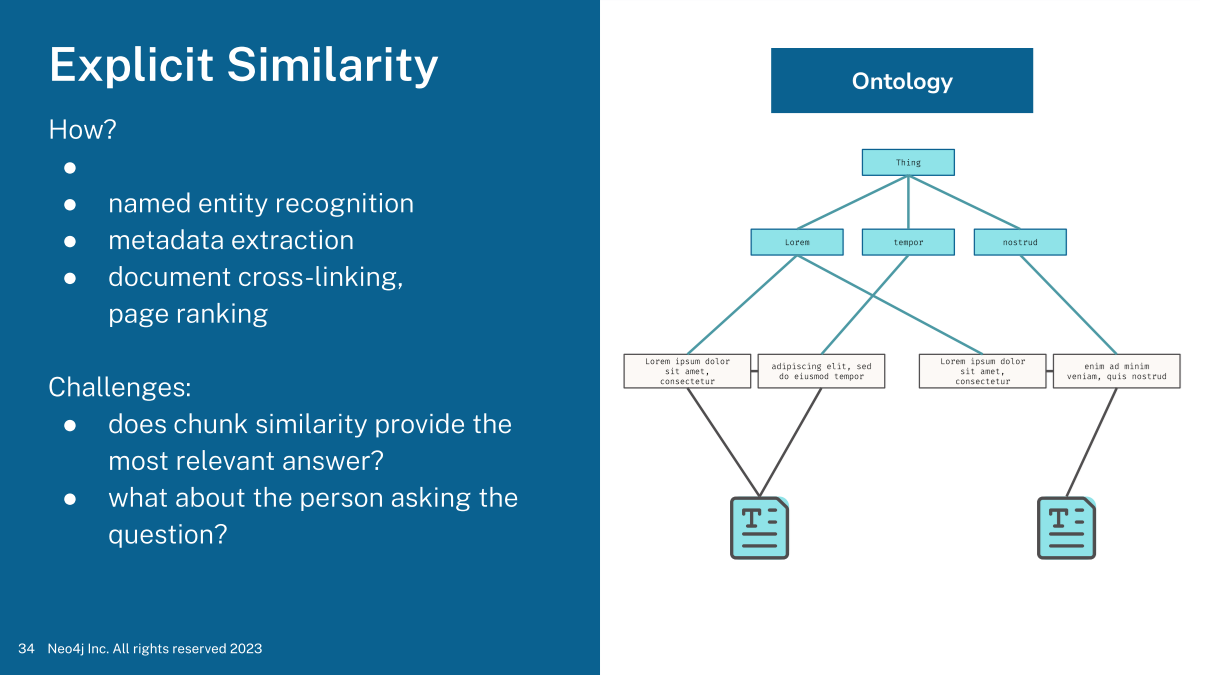
\includegraphics[width=\linewidth,keepaspectratio]{graphrag5}
	\end{center}
	
\end{frame}

%%%%%%%%%%%%%%%%%%%%%%%%%%%%%%%%%%%%%%%%%%%%%%%%%%%%%%%%%%%
\begin{frame}[fragile]\frametitle{}

	\begin{center}
	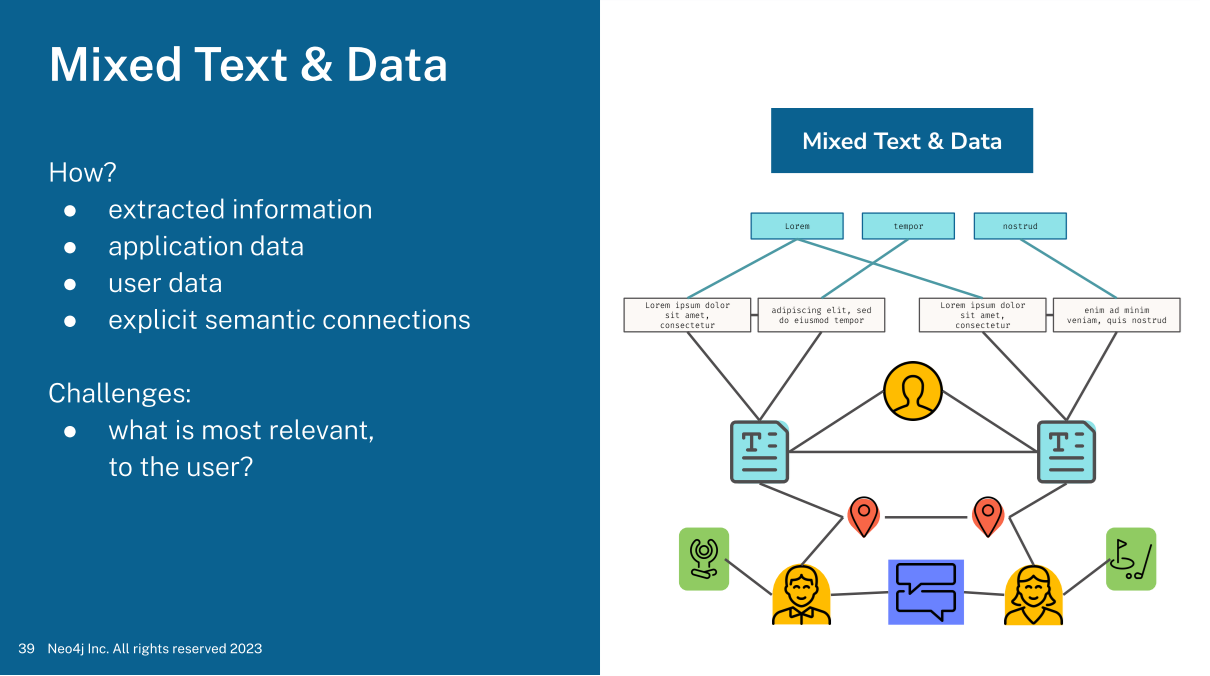
\includegraphics[width=\linewidth,keepaspectratio]{graphrag6}
	\end{center}
	
\end{frame}





% %%%%%%%%%%%%%%%%%%%%%%%%%%%%%%%%%%%%%%%%%%%%%%%%%%%%%%%%%%%
% \begin{frame}[fragile]\frametitle{}

	% \begin{center}
	% 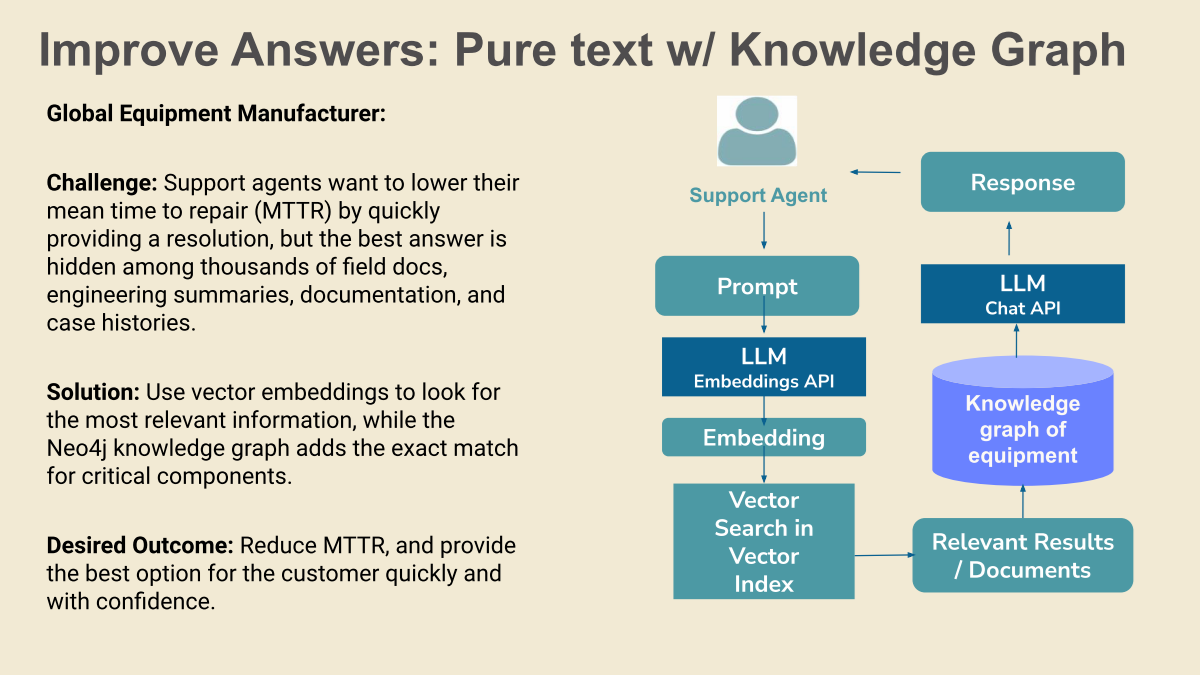
\includegraphics[width=\linewidth,keepaspectratio]{graphrag8}
	% \end{center}
	
% \end{frame}


% %%%%%%%%%%%%%%%%%%%%%%%%%%%%%%%%%%%%%%%%%%%%%%%%%%%%%%%%%%%
% \begin{frame}[fragile]\frametitle{}

	% \begin{center}
	% 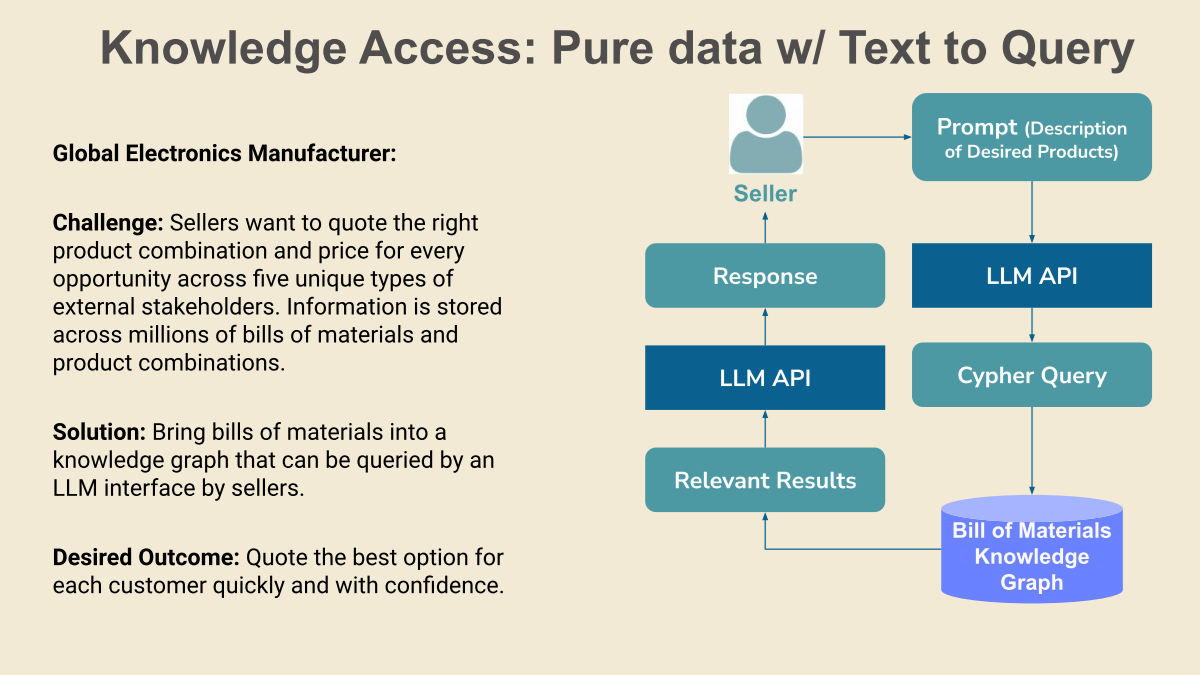
\includegraphics[width=\linewidth,keepaspectratio]{graphrag9}
	% \end{center}
	
% \end{frame}

% %%%%%%%%%%%%%%%%%%%%%%%%%%%%%%%%%%%%%%%%%%%%%%%%%%%%%%%%%%%
% \begin{frame}[fragile]\frametitle{}

	% \begin{center}
	% 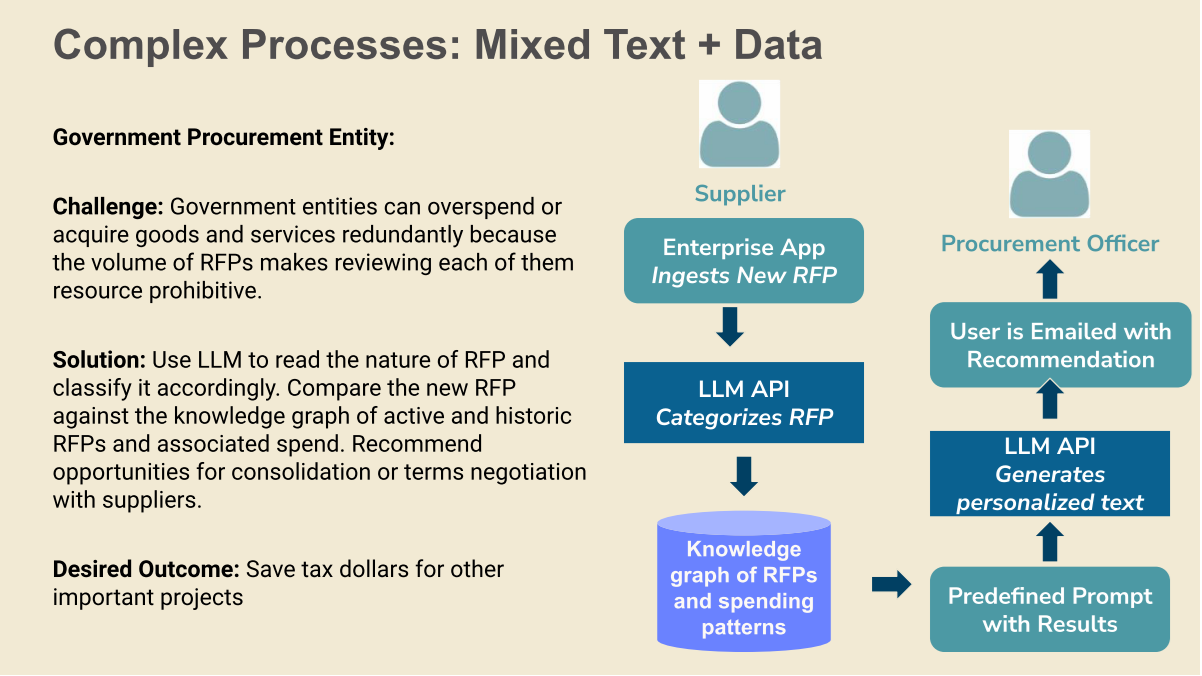
\includegraphics[width=\linewidth,keepaspectratio]{graphrag10}
	% \end{center}
	
% \end{frame}

%%%%%%%%%%%%%%%%%%%%%%%%%%%%%%%%%%%%%%%%%%%%%%%%%%%%%%%%%%%
\begin{frame}[fragile]\frametitle{Conclusion}
    \begin{itemize}
        \item GraphRAG scales from local to global knowledge representation.
        \item Community-based summaries improve response quality.
        \item Enables optimized retrieval with hierarchical partitioning.
    \end{itemize}
\end{frame}


%%%%%%%%%%%%%%%%%%%%%%%%%%%%%%%%%%%%%%%%%%%%%%%%%%%%%%%%%%%%%%%%%%%%%%%%%%%%%%%%%%
\begin{frame}[fragile]\frametitle{}
\begin{center}
{\Large Graph RAG for Agents}

{\tiny (Ref: LinkedIn post by Maryam Miradi)}

\end{center}
\end{frame}


%%%%%%%%%%%%%%%%%%%%%%%%%%%%%%%%%%%%%%%%%%%%%%%%%%%%%%%%%%%
\begin{frame}[fragile]\frametitle{The Future is Clear: Why Agents Need Graph RAG}
      \begin{itemize}
        \item Graph RAG combines multi-hop reasoning capabilities with advanced retrieval
        \item Utilizes non-parameterized and learning-based retrieval methods
        \item Implements topology-aware prompting to preserve knowledge structure
        \item Addresses core LLM limitations: hallucinations, forgetting, complex reasoning
      \end{itemize}
\end{frame}

%%%%%%%%%%%%%%%%%%%%%%%%%%%%%%%%%%%%%%%%%%%%%%%%%%%%%%%%%%%
\begin{frame}[fragile]\frametitle{What Is Graph-Enhanced RAG?}
      \begin{itemize}
        \item LLMs struggle with hallucinations, memory limitations, and complex reasoning
        \item Graphs organize knowledge into structured networks of connected facts
        \item Knowledge graphs provide explicit relationships between entities
        \item Graph RAG enables LLMs to follow logical paths rather than guess
        \item Results in more factual, coherent, and logically sound responses
      \end{itemize}
\end{frame}

%%%%%%%%%%%%%%%%%%%%%%%%%%%%%%%%%%%%%%%%%%%%%%%%%%%%%%%%%%%
\begin{frame}[fragile]\frametitle{The 4-Step Workflow of Graph RAG}
      \begin{itemize}
        \item \textbf{User Query}: Initial question or request from user
        \item \textbf{Retrieval Module}: Fetches structurally relevant knowledge from graph
        \item \textbf{Prompting Module}: Reshapes retrieved knowledge into optimal prompt format
        \item \textbf{Output Response}: LLM generates fact-rich, logically sound answer
        \item Example: "How did Einstein use Riemannian geometry?" retrieves Einstein, Grossmann, and Riemannian Geometry entities
      \end{itemize}
\end{frame}

%%%%%%%%%%%%%%%%%%%%%%%%%%%%%%%%%%%%%%%%%%%%%%%%%%%%%%%%%%%
\begin{frame}[fragile]\frametitle{Step 1: Build Graph-Powered Databases}
      \begin{itemize}
        \item \textbf{Use Existing Knowledge Graphs}:
          \begin{itemize}
            \item Freebase, Wikidata
            \item Structured and reliable, but static
          \end{itemize}
        \item \textbf{Build New Graphs From Text}:
          \begin{itemize}
            \item Using OpenIE or instruction-tuned LLMs
            \item Dynamic and adaptable, but potentially messy
          \end{itemize}
      \end{itemize}
\end{frame}

%%%%%%%%%%%%%%%%%%%%%%%%%%%%%%%%%%%%%%%%%%%%%%%%%%%%%%%%%%%
\begin{frame}[fragile]\frametitle{Step 2: Retrieval Algorithms}
      \begin{itemize}
        \item \textbf{Non-Parameterized Retrieval}:
          \begin{itemize}
            \item Deterministic, probabilistic, and heuristic approaches
            \item Examples: Dijkstra's algorithm, PageRank, 1-hop neighbors
            \item Fast but rigid in operation
          \end{itemize}
        \item \textbf{Learning-Based Retrieval}:
          \begin{itemize}
            \item Graph Neural Networks (GNNs), Attention Models
            \item Graph convolution and graph attention techniques
            \item Smarter and deeper, but computationally heavier
          \end{itemize}
      \end{itemize}
\end{frame}

%%%%%%%%%%%%%%%%%%%%%%%%%%%%%%%%%%%%%%%%%%%%%%%%%%%%%%%%%%%
\begin{frame}[fragile]\frametitle{Step 2: Prompting Approaches}
      \begin{itemize}
        \item \textbf{Topology-Aware Prompting}:
          \begin{itemize}
            \item Preserves graph structure in prompts
            \item Enables multi-hop reasoning capabilities
            \item Maintains relationship context
          \end{itemize}
        \item \textbf{Text Prompting}:
          \begin{itemize}
            \item Flattens graph data into readable sentences
            \item More suitable for vanilla LLMs
            \item Easier to process but may lose structural information
          \end{itemize}
      \end{itemize}
\end{frame}

%%%%%%%%%%%%%%%%%%%%%%%%%%%%%%%%%%%%%%%%%%%%%%%%%%%%%%%%%%%
\begin{frame}[fragile]\frametitle{Step 3: Graph-Structured Pipelines}
      \begin{itemize}
        \item \textbf{Sequential Pipelines}:
          \begin{itemize}
            \item Straightforward flow: query → retrieve → prompt → answer
            \item Simple and efficient for basic questions
          \end{itemize}
        \item \textbf{Loop Pipelines}:
          \begin{itemize}
            \item Iterative refinement until optimal evidence is found
            \item Self-correcting and precision-focused
          \end{itemize}
        \item \textbf{Tree Pipelines}:
          \begin{itemize}
            \item Parallel exploration of multiple knowledge paths
            \item More comprehensive for complex queries
          \end{itemize}
      \end{itemize}
\end{frame}

%%%%%%%%%%%%%%%%%%%%%%%%%%%%%%%%%%%%%%%%%%%%%%%%%%%%%%%%%%%
\begin{frame}[fragile]\frametitle{Step 4: Graph-Oriented Tasks}
      \begin{itemize}
        \item \textbf{Knowledge Graph QA (KGQA)}:
          \begin{itemize}
            \item Answering deep, logical questions using graph structures
            \item Enables complex queries across multiple knowledge domains
          \end{itemize}
        \item \textbf{Graph-Specific Tasks}:
          \begin{itemize}
            \item Node classification, link prediction, graph summarization
            \item Structural analysis and pattern recognition
          \end{itemize}
        \item \textbf{Domain-Specific Applications}:
          \begin{itemize}
            \item Specialized use in biomedicine, law, scientific discovery, finance
            \item Enables domain-specific reasoning with expert knowledge
          \end{itemize}
      \end{itemize}
\end{frame}

%%%%%%%%%%%%%%%%%%%%%%%%%%%%%%%%%%%%%%%%%%%%%%%%%%%%%%%%%%%
\begin{frame}[fragile]\frametitle{Conclusion: Benefits of Graph RAG}
      \begin{itemize}
        \item Significantly reduces hallucinations through structured knowledge
        \item Enhances multi-hop reasoning capabilities for complex queries
        \item Improves explainability with transparent knowledge paths
        \item Enables domain-specific expertise through specialized knowledge graphs
        \item Represents the future of reliable, reasoning-based AI agents
      \end{itemize}
\end{frame}








